\section{Tworzenie i testowanie API REST w .NET}

\subsection{Wprowadzenie do API REST}
REST (Representational State Transfer) to architektura, która definiuje zasady komunikacji między klientem a serwerem przy użyciu protokołu HTTP.  
W .NET API REST jest zwykle budowane przy użyciu \texttt{ASP.NET Core Web API}, co umożliwia szybkie tworzenie usług sieciowych, które komunikują się w formacie JSON.

\subsection{Tworzenie projektu Web API}
Nowy projekt można utworzyć poleceniem:
\begin{lstlisting}[language=bash, caption={Tworzenie projektu Web API w .NET}]
dotnet new webapi -n ShopAPI.Api
cd ShopAPI.Api
dotnet run
\end{lstlisting}

Po uruchomieniu aplikacji interfejs testowy Swagger jest dostępny pod adresem:
\begin{center}
\texttt{https://localhost:7294/swagger/index.html}
\end{center}

\subsection{Certyfikaty HTTPS i zaufanie lokalne}
Domyślnie .NET generuje certyfikat deweloperski HTTPS.  
Jeżeli przeglądarka zgłasza problem z zaufaniem, można go zarejestrować:
\begin{lstlisting}[language=bash, caption={Rejestracja certyfikatu deweloperskiego}]
dotnet dev-certs https --trust
\end{lstlisting}

\subsection{Testowanie API}
Istnieje wiele sposobów testowania API:
\begin{itemize}
    \item \textbf{Swagger} – interaktywny interfejs do testów,
    \item \textbf{curl} – narzędzie wiersza poleceń,
    \item \textbf{Postman} – aplikacja GUI do testów HTTP,
    \item \textbf{Pliki .http} – zintegrowane z Visual Studio Code,
    \item \textbf{Przeglądarka} – do zapytań GET.
\end{itemize}

\begin{lstlisting}[language=bash, caption={Przykładowe zapytanie curl}]
curl -X GET https://localhost:7294/api/cities
\end{lstlisting}

\subsection{Czasowniki HTTP i ich zastosowanie}
\begin{center}
\begin{tabular}{|l|l|l|}
\hline
\textbf{Metoda} & \textbf{Opis} & \textbf{Przykład} \\
\hline
GET & Pobranie danych & /api/cities \\
POST & Dodanie nowych danych & /api/cities \\
PUT & Nadpisanie danych & /api/cities/3 \\
PATCH & Częściowa aktualizacja & /api/cities/3 \\
DELETE & Usunięcie danych & /api/cities/3 \\
\hline
\end{tabular}
\end{center}

\subsection{Tworzenie modelu danych i DTO}
\textbf{Model} reprezentuje dane domenowe, natomiast \textbf{DTO} (Data Transfer Object) służy do przesyłania danych między klientem a API.

\begin{lstlisting}[language=C, caption={Przykładowy model City}]
public class City
{
    public int Id { get; set; }
    public string Name { get; set; } = string.Empty;
    public int Population { get; set; }
}
\end{lstlisting}

\begin{lstlisting}[language=C, caption={Przykładowy DTO CityDto}]
public class CityDto
{
    public string Name { get; set; } = string.Empty;
    public int Population { get; set; }
}
\end{lstlisting}

\subsection{Implementacja kontrolera}
\begin{lstlisting}[language=C, caption={Kontroler CitiesController}]
[ApiController]
[Route("api/[controller]")]
public class CitiesController : ControllerBase
{
    private static List<City> _cities = new()
    {
        new City { Id = 1, Name = "Warszawa", Population = 1790658 },
        new City { Id = 2, Name = "Kraków", Population = 800653 }
    };

    [HttpGet]
    public ActionResult<IEnumerable<CityDto>> GetCities()
        => Ok(_cities.Select(c => new CityDto
        {
            Name = c.Name,
            Population = c.Population
        }));

    [HttpGet("{id}")]
    public ActionResult<CityDto> GetCity(int id)
    {
        var city = _cities.FirstOrDefault(c => c.Id == id);
        if (city == null)
            return NotFound();
        return Ok(new CityDto { Name = city.Name, Population = city.Population });
    }

    [HttpPost]
    public ActionResult<CityDto> CreateCity(CityDto dto)
    {
        if (_cities.Any(c => c.Name == dto.Name))
            return Conflict("City already exists.");

        var city = new City
        {
            Id = _cities.Max(c => c.Id) + 1,
            Name = dto.Name,
            Population = dto.Population
        };
        _cities.Add(city);
        return CreatedAtAction(nameof(GetCity), new { id = city.Id }, dto);
    }
}
\end{lstlisting}
\section*{Znaczenie kodów statusu HTTP}

\begin{center}
	\begin{tabular}{>{\bfseries}c m{4cm} m{7cm}}
		\toprule
		Zakres kodów & Znaczenie & Opis \\
		\midrule
		1xx & Informacyjne (Informational) & Serwer przyjął żądanie i przetwarza je dalej. Rzadko widoczne dla użytkownika. \\
		2xx & Sukces (Success) & Żądanie zostało pomyślnie wykonane. Najczęstszy: \texttt{200 OK}. \\
		3xx & Przekierowanie (Redirection) & Wymaga dodatkowego działania, np. przekierowania na inny adres (\texttt{301 Moved Permanently}, \texttt{302 Found}). \\
		4xx & Błąd po stronie klienta (Client Error) & Coś nie tak z zapytaniem użytkownika (\texttt{404 Not Found}, \texttt{403 Forbidden}). \\
		5xx & Błąd po stronie serwera (Server Error) & Serwer ma problem z przetworzeniem żądania (\texttt{500 Internal Server Error}, \texttt{503 Service Unavailable}). \\
		\bottomrule
	\end{tabular}
\end{center}

\subsection{Kody odpowiedzi HTTP}
Najczęściej używane kody odpowiedzi:
\begin{itemize}
    \item 200 OK – żądanie wykonano poprawnie,
    \item 201 Created – obiekt został utworzony,
    \item 204 No Content – brak treści w odpowiedzi,
    \item 400 Bad Request – błędne żądanie,
    \item 401 Unauthorized – brak autoryzacji,
    \item 403 Forbidden – brak dostępu,
    \item 404 Not Found – zasób nie istnieje,
    \item 409 Conflict – konflikt danych,
    \item 500 Internal Server Error – błąd serwera.
\end{itemize}

\subsection{Generowanie klienta z OpenAPI / Swagger}
\textbf{Swagger} umożliwia wygenerowanie klienta API w wielu językach, np. przez narzędzie \texttt{NSwag}:
\begin{lstlisting}[language=bash]
nswag openapi2csclient /input:https://localhost:7294/swagger/v1/swagger.json /output:CitiesClient.cs
\end{lstlisting}

Taki klient może być wykorzystany w aplikacji konsolowej, WPF lub MAUI:
\begin{lstlisting}[language=C]
var client = new CitiesClient("https://localhost:7294", new HttpClient());
var cities = await client.GetCitiesAsync();
\end{lstlisting}

\subsection{Autentykacja i autoryzacja}
Wspierane są standardy:
\begin{itemize}
    \item OAuth 2.0,
    \item OpenID Connect,
    \item Entra ID (Azure AD),
    \item Google Identity.
\end{itemize}

\subsection{Walidacja, idempotencja i paginacja}
\begin{itemize}
    \item Walidacja danych wejściowych przy użyciu \texttt{DataAnnotations},
    \item Idempotencja – operacje powinny dawać ten sam wynik przy wielokrotnym wywołaniu (np. PUT),
    \item Paginacja – ograniczenie liczby wyników (np. \texttt{/api/cities?page=2\&size=10}).
\end{itemize}

\subsection{Diagram przepływu zapytania REST API}
\begin{center}
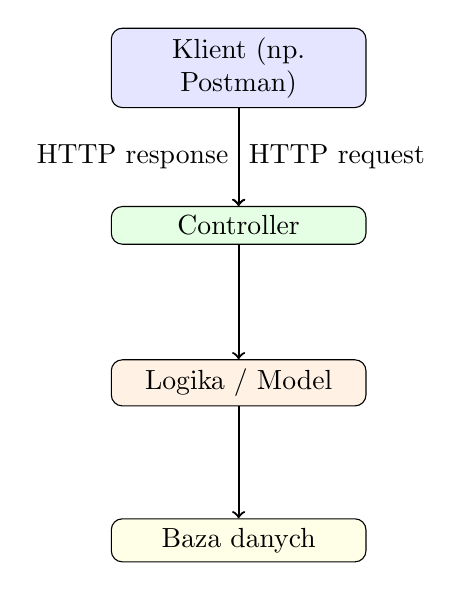
\begin{tikzpicture}[node distance=2cm, every node/.style={align=center}]
\node (client) [draw, rounded corners, fill=blue!10, text width=3cm] {Klient (np. Postman)};
\node (controller) [draw, rounded corners, fill=green!10, below of=client, text width=3cm] {Controller};
\node (service) [draw, rounded corners, fill=orange!10, below of=controller, text width=3cm] {Logika / Model};
\node (db) [draw, rounded corners, fill=yellow!10, below of=service, text width=3cm] {Baza danych};

\draw[->, thick] (client) -- node[right]{HTTP request} (controller);
\draw[->, thick] (controller) -- (service);
\draw[->, thick] (service) -- (db);
\draw[<- ,thick] (controller) -- node[left]{HTTP response} (client);
\end{tikzpicture}
\end{center}

\subsection{HEAD i OPTIONS - dodatkowe metody HTTP}
Oprócz podstawowych metod GET, POST, PUT, PATCH i DELETE, REST API wspiera również:

\begin{lstlisting}[language=C, caption={Implementacja HEAD i OPTIONS}]
	[HttpHead("{id}")]
	public IActionResult CheckCityExists(int id)
	{
		var exists = _cities.Any(c => c.Id == id);
		return exists ? Ok() : NotFound();
	}
	
	[HttpOptions]
	public IActionResult GetCitiesOptions()
	{
		Response.Headers.Add("Allow", "GET, POST, PUT, PATCH, DELETE, HEAD, OPTIONS");
		return Ok();
	}
\end{lstlisting}

\begin{itemize}
	\item \textbf{HEAD} -- sprawdza istnienie zasobu bez pobierania treści (zwraca tylko nagłówki),
	\item \textbf{OPTIONS} -- zwraca listę dostępnych metod HTTP dla danego endpointu.
\end{itemize}

\subsection{OAuth 2.0 i OpenID Connect -- szczegółowy flow}
\subsubsection{Authorization Code + PKCE Flow}
PKCE (Proof Key for Code Exchange) to rozszerzenie OAuth 2.0 zapewniające bezpieczeństwo dla aplikacji publicznych (SPA, mobile).

\textbf{Krok 1: Generowanie PKCE}
\begin{itemize}
	\item \texttt{code\_verifier} -- losowy string 43-128 znaków (Base64URL)
	\item \texttt{code\_challenge} -- Base64URL(SHA256(code\_verifier))
	\item \texttt{code\_challenge\_method} -- "S256" (SHA-256)
\end{itemize}

\textbf{Krok 2: Żądanie autoryzacji (redirect do przeglądarki)}
\begin{lstlisting}[language=bash]
	GET https://login.microsoftonline.com/{tenant}/oauth2/v2.0/authorize
	?client_id=<APP_ID>
	&response_type=code
	&redirect_uri=<REDIRECT_URI>
	&scope=openid profile email offline_access
	&code_challenge=<CHALLENGE>
	&code_challenge_method=S256
	&state=<RANDOM_STATE>
\end{lstlisting}

\textbf{Krok 3: Wymiana kodu na token}
\begin{lstlisting}[language=bash]
	POST https://login.microsoftonline.com/{tenant}/oauth2/v2.0/token
	Content-Type: application/x-www-form-urlencoded
	
	grant_type=authorization_code
	&code=<AUTHORIZATION_CODE>
	&redirect_uri=<REDIRECT_URI>
	&client_id=<APP_ID>
	&code_verifier=<VERIFIER>
\end{lstlisting}

\textbf{Odpowiedź:}
\begin{lstlisting}[language=json]
	{
		"access_token": "eyJ0eXAiOiJKV1...",
		"id_token": "eyJ0eXAiOiJKV1...",
		"refresh_token": "0.AXoA...",
		"token_type": "Bearer",
		"expires_in": 3600
	}
\end{lstlisting}

\subsubsection{Konfiguracja providerów}
\textbf{Google (Google Cloud Console):}
\begin{itemize}
	\item Authorize endpoint: \texttt{https://accounts.google.com/o/oauth2/v2/auth}
	\item Token endpoint: \texttt{https://oauth2.googleapis.com/token}
	\item Scope: \texttt{openid email profile}
	\item Redirect URI: np. \texttt{https://localhost:7294/signin-oidc}
\end{itemize}

\textbf{Microsoft Entra ID (Azure Portal):}
\begin{itemize}
	\item Tenant ID -- z "Directory (tenant) ID"
	\item Application (client) ID -- z "App registrations"
	\item Authorize endpoint: \texttt{https://login.microsoftonline.com/\{tenant\}/oauth2/v2.0/authorize}
	\item Token endpoint: \texttt{https://login.microsoftonline.com/\{tenant\}/oauth2/v2.0/token}
	\item Scope: \texttt{openid profile email} (+ \texttt{offline\_access} dla refresh token)
\end{itemize}

\subsubsection{Integracja w .NET API}
\begin{lstlisting}[language=C, caption={Konfiguracja JWT Bearer w Minimal API}]
	builder.Services.AddAuthentication(JwtBearerDefaults.AuthenticationScheme)
	.AddJwtBearer(options =>
	{
		options.Authority = "https://login.microsoftonline.com/{tenant}/v2.0";
		options.Audience = "{CLIENT_ID}";
		options.TokenValidationParameters = new TokenValidationParameters
		{
			ValidateIssuer = true,
			ValidateAudience = true,
			ValidateLifetime = true
		};
	});
	
	app.UseAuthentication();
	app.UseAuthorization();
	
	// Zabezpieczony endpoint
	app.MapGet("/api/secure", [Authorize] () => "Authenticated!")
	.RequireAuthorization();
\end{lstlisting}

\subsection{Paginacja i filtrowanie}
\begin{lstlisting}[language=C, caption={Przykład paginacji w kontrolerze}]
	[HttpGet]
	public ActionResult<IEnumerable<CityDto>> GetCities(
	[FromQuery] int page = 1, 
	[FromQuery] int pageSize = 10,
	[FromQuery] string? country = null)
	{
		var query = _cities.AsQueryable();
		
		// Filtrowanie
		if (!string.IsNullOrEmpty(country))
		query = query.Where(c => c.Country == country);
		
		// Paginacja
		var total = query.Count();
		var items = query
		.Skip((page - 1) * pageSize)
		.Take(pageSize)
		.Select(c => new CityDto { Name = c.Name, Country = c.Country });
		
		Response.Headers.Add("X-Total-Count", total.ToString());
		return Ok(items);
	}
\end{lstlisting}

Przykład użycia: \texttt{GET /api/cities?page=2\&pageSize=5\&country=Poland}

\subsection{Idempotencja metod HTTP}
\textbf{Idempotencja} oznacza, że wielokrotne wywołanie tej samej operacji daje ten sam efekt co pojedyncze wywołanie.

\begin{center}
	\begin{tabular}{|l|l|l|}
		\hline
		\textbf{Metoda} & \textbf{Idempotentna?} & \textbf{Wyjaśnienie} \\
		\hline
		GET & Tak & Wielokrotne pobranie nie zmienia stanu \\
		POST & Nie & Każde wywołanie tworzy nowy zasób \\
		PUT & Tak & Nadpisanie tym samym daje ten sam stan \\
		PATCH & Zależy & Może być idempotentna (zależy od implementacji) \\
		DELETE & Tak & Usunięcie już usuniętego zwraca 404, ale stan się nie zmienia \\
		\hline
	\end{tabular}
\end{center}

\subsection{HATEOAS (Hypermedia As The Engine Of Application State)}
HATEOAS to zasada REST, która polega na zwracaniu w odpowiedzi linków do powiązanych zasobów.

\begin{lstlisting}[language=C, caption={Przykład HATEOAS}]
	[HttpGet("{id}")]
	public ActionResult<CityWithLinks> GetCity(int id)
	{
		var city = _cities.FirstOrDefault(c => c.Id == id);
		if (city == null) return NotFound();
		
		return Ok(new
		{
			city.Id,
			city.Name,
			city.Country,
			_links = new
			{
				self = Url.Action(nameof(GetCity), new { id }),
				update = Url.Action(nameof(UpdateCity), new { id }),
				delete = Url.Action(nameof(DeleteCity), new { id }),
				all = Url.Action(nameof(GetCities))
			}
		});
	}
\end{lstlisting}

Odpowiedź JSON:
\begin{lstlisting}[language=json]
	{
		"id": 1,
		"name": "Warszawa",
		"country": "Poland",
		"_links": {
			"self": "/api/cities/1",
			"update": "/api/cities/1",
			"delete": "/api/cities/1",
			"all": "/api/cities"
		}
	}
\end{lstlisting}

\subsection{Podsumowanie rozdziału}
\begin{itemize}
    \item API REST w .NET jest oparte o architekturę HTTP i format JSON.
    \item Kontrolery mapują żądania na metody akcji.
    \item Swagger pozwala testować i generować klienta.
    \item Kluczowe są poprawne kody HTTP i walidacja danych.
    \item Uwierzytelnianie i autoryzacja zapewniają bezpieczeństwo aplikacji.
\end{itemize}

\subsection{Pytania kontrolne}
\begin{enumerate}
    \item Jakie są główne metody HTTP używane w REST API?
    \item Czym różni się model od DTO?
    \item Jak można przetestować API bez użycia Postmana?
    \item Jakie są typowe kody błędów HTTP?
    \item Do czego służy narzędzie NSwag?
\end{enumerate}
